% ============================================================
%  ETSIIT Smart Campus — Presentación (Beamer, 16:9)
%  Compilar con:  pdflatex presentacion.tex  (dos veces)
%  Los recuadros discontinuos "CAPTURA" son huecos para imágenes.
%  Para sustituirlos: cambia \ph{ancho}{alto}{texto} por
%  \includegraphics[width=ancho]{fichero.png}
% ============================================================
\documentclass[aspectratio=169,11pt]{beamer}

\usepackage[utf8]{inputenc}
\usepackage[T1]{fontenc}
\usepackage[scaled=0.92]{helvet}
\usepackage{tikz}
\usepackage{graphicx}
\usetikzlibrary{positioning,arrows.meta,calc,shapes.geometric}

% ---------- Colores ----------
\definecolor{granate}{HTML}{9B1B30}
\definecolor{azul}{HTML}{1F4E9C}
\definecolor{verde}{HTML}{2E8B57}
\definecolor{ink}{HTML}{2B2B2B}
\definecolor{panel}{HTML}{F5F1F2}

% ---------- Tema ----------
\usetheme{default}
\renewcommand{\familydefault}{\sfdefault}
\setbeamercolor{normal text}{fg=ink}
\setbeamertemplate{navigation symbols}{}
\setbeamersize{text margin left=10mm,text margin right=10mm}
\setbeamerfont{itemize/enumerate body}{size=\small}
\setbeamertemplate{itemize item}{\raisebox{0.25ex}{\color{granate}\vrule width 3.5pt height 3.5pt}}
\setbeamertemplate{itemize subitem}{\raisebox{0.25ex}{\color{granate}\vrule width 2.5pt height 2.5pt}}
\setlength{\leftmargini}{1.1em}

\setbeamertemplate{background}{%
  \begin{tikzpicture}[remember picture,overlay]
    \fill[granate] (current page.north west) rectangle ([yshift=-2.5mm]current page.north east);
  \end{tikzpicture}}

\setbeamertemplate{frametitle}{%
  \vspace{3.5mm}\hspace{-1mm}%
  {\color{granate}\rule[-1.2mm]{3.5pt}{6.5mm}}\hspace{2.5mm}%
  {\Large\bfseries\color{granate!85!black}\insertframetitle}\par\vspace{1mm}}

\setbeamertemplate{footline}{%
  \begin{tikzpicture}[remember picture,overlay]
    \node[anchor=south west,font=\tiny,text=gray] at ($(current page.south west)+(10mm,3mm)$)
      {ETSIIT Smart Campus \textperiodcentered{} Nuevos Paradigmas de Interacción 2026--27};
    \node[anchor=south east,font=\tiny,text=gray] at ($(current page.south east)+(-10mm,3mm)$)
      {\insertframenumber\,/\,\inserttotalframenumber};
  \end{tikzpicture}}

% ---------- Macros ----------
% Hueco para captura: \ph{ancho}{alto}{descripción}
\newcommand{\ph}[3]{%
  \begin{tikzpicture}
    \node[draw=granate!60,dashed,thick,rounded corners=4pt,fill=granate!5,
          inner sep=3pt,font=\scriptsize\color{granate},align=center]
      {\parbox[c][#2][c]{#1}{\centering\textbf{[CAPTURA]}\\[1pt]#3}};
  \end{tikzpicture}}

% Tarjeta: \card{ancho}{alto}{color}{título}{texto}
\newcommand{\card}[5]{%
  \begin{tikzpicture}
    \node[draw=#3,fill=#3!6,rounded corners=5pt,line width=0.8pt,inner sep=6pt]
      {\parbox[t][#2][t]{#1}{\raggedright{\bfseries\color{#3}#4}\\[3pt]\footnotesize #5}};
  \end{tikzpicture}}

% Insignia de demo (arriba a la derecha)
\newcommand{\demo}{%
  \begin{tikzpicture}[remember picture,overlay]
    \node[anchor=north east,fill=verde,text=white,rounded corners=7pt,
          inner xsep=8pt,inner ysep=3pt,font=\scriptsize\bfseries]
      at ($(current page.north east)+(-10mm,-8.5mm)$) {DEMO EN LA APP};
  \end{tikzpicture}}

% Quién presenta (abajo a la derecha)
\newcommand{\presenta}[1]{%
  \begin{tikzpicture}[remember picture,overlay]
    \node[anchor=south east,fill=azul!12,text=azul,rounded corners=7pt,
          inner xsep=7pt,inner ysep=2.5pt,font=\tiny\bfseries]
      at ($(current page.south east)+(-22mm,2.3mm)$) {Presenta: #1};
  \end{tikzpicture}}

\newcommand{\code}[1]{{\ttfamily\color{azul}#1}}

\title{ETSIIT Smart Campus}
\author{}
\date{}

\tikzset{
  step/.style={draw=#1,fill=#1!8,rounded corners=6pt,line width=1pt,
    minimum width=19mm,minimum height=13mm,align=center,font=\footnotesize},
  st/.style={draw=#1,fill=#1!8,rounded corners=5pt,line width=1pt,
    minimum width=29mm,minimum height=13mm,align=center,font=\scriptsize},
  layer/.style={draw=#1,fill=#1!8,rounded corners=4pt,line width=0.9pt,
    minimum width=7.4cm,minimum height=9mm,align=left,font=\scriptsize,inner xsep=8pt}}
\begin{document}

% ============================================================
%  PORTADA
% ============================================================
{\setbeamercolor{background canvas}{bg=granate!90!black}
\begin{frame}[plain]
  \begin{tikzpicture}[remember picture,overlay,text=white]
    % Logo UGR
    \node[anchor=north west] at ($(current page.north west)+(12mm,-5mm)$)
        {{
\includegraphics[width=12mm]{img/logo_ugr_white.png}}};
    \node[anchor=north west,text=white,font=\footnotesize,align=left]
      at ($(current page.north west)+(26mm,-7mm)$)
      {{Universidad de Granada}\\[3pt]ETSIIT};

    % Título
    \node[anchor=west,align=left,text width=95mm] at ($(current page.west)+(12mm,7mm)$)
      {{\fontsize{30}{34}\selectfont\bfseries ETSIIT\\Smart Campus}\\[5mm]
       {\large Guía de orientación por la ETSIIT\\con sensores en Android}};
    \draw[white,line width=1.2pt] ($(current page.west)+(42mm,-22mm)$) -- ++(30mm,0);

    % Autores
    \node[anchor=south west,align=left,font=\scriptsize,text width=90mm, align=center]
      at ($(current page.south west)+(12mm,10mm)$)
        {%
            Jesús Muñoz Velasco \textperiodcentered{} 
            Juan Antonio Galindo Benítez \\
            José Manuel Sánchez Varbas \textperiodcentered{} 
            Daniel Morán Sánchez \\
            Miguel Gangoso Martínez%
        };

    % Captura
    \node[anchor=east,thick,rounded corners=10pt,fill=granate!90!white,
          minimum width=42mm,minimum height=82mm]
      at ($(current page.east)+(-5mm,-2mm)$) {};

    \node[anchor=east, inner sep=0pt] 
        at ($(current page.east)+(-6.75mm,-2mm)$)
        {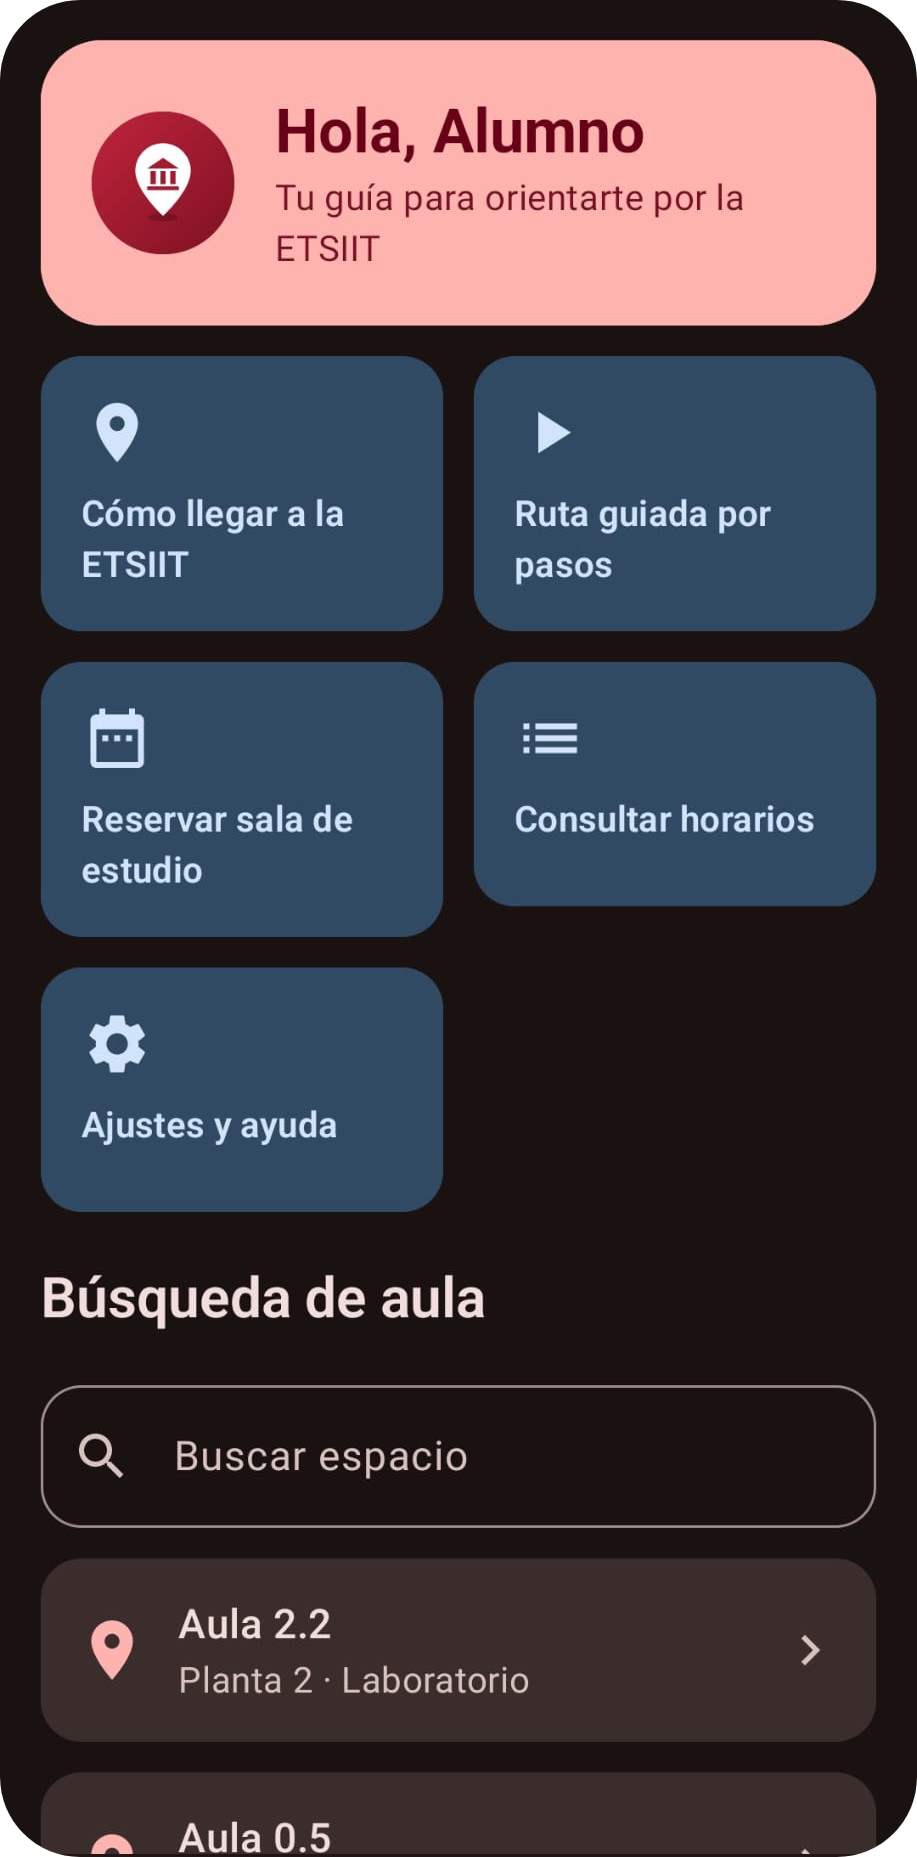
\includegraphics[height=78mm]{img/pagina_inicio.png}};
    
    % Asignatura
    \node[anchor=south west, align=center, text width=90mm] at ($(current page.south west)+(12mm,3mm)$) 
    {\fontsize{7}{9}\selectfont Nuevos Paradigmas de Interacción \textperiodcentered{} 2026--27 \textperiodcentered{} Granada, noviembre de 2026};
    
  \end{tikzpicture}
\end{frame}}

% ============================================================
%  1. EL PROBLEMA Y LA IDEA
% ============================================================
\begin{frame}{El problema y la idea}
  \begin{columns}[T]
    \column{0.47\textwidth}
      {\Large\bfseries ¿Cómo llego al aula 2.2?}\\[4mm]
      \begin{itemize}\setlength\itemsep{4pt}
        \item El GPS necesita ver al menos 4 satélites y tiene ${\approx}15$\,m de error: \textbf{no sirve dentro de un edificio}.
        \item No hay posicionamiento interior.
        \item La ruta solo avanza cuando \textbf{el usuario lo confirma}: QR, NFC o ``Ya estoy aquí''.
        \item Nunca avanza por una estimación de los sensores.
      \end{itemize}
    \column{0.50\textwidth}
      \vspace{2mm}
      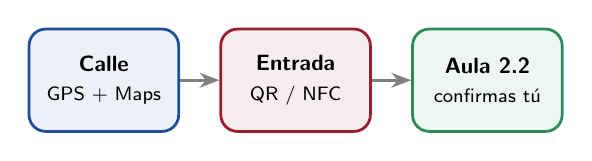
\begin{tikzpicture}[
          arr/.style={-{Stealth[length=2.5mm]},line width=1.2pt,gray}]
        \node[step=azul] (a) {\textbf{Calle}\\[1pt]\scriptsize GPS + Maps};
        \node[step=granate,right=5mm of a] (b) {\textbf{Entrada}\\[1pt]\scriptsize QR / NFC};
        \node[step=verde,right=5mm of b] (c) {\textbf{Aula 2.2}\\[1pt]\scriptsize confirmas tú};
        \draw[arr] (a)--(b); \draw[arr] (b)--(c);
      \end{tikzpicture}
      \\[7mm]
      \begin{tikzpicture}
        \node[fill=granate,text=white,rounded corners=8pt,inner xsep=10pt,inner ysep=8pt,
              text width=62mm,align=center]
          {{\large\bfseries «La app orienta, no localiza»}\\[3pt]
           \footnotesize Los sensores ayudan, pero nunca afirman dónde está el usuario};
      \end{tikzpicture}
  \end{columns}
  \presenta{Jesús}
\end{frame}

% ============================================================
%  2. RECORRIDO DE USO
% ============================================================
\begin{frame}{De la calle al aula}
  \centering
  \begin{tikzpicture}[arr/.style={-{Stealth[length=2mm]},line width=1pt,gray}]
    \foreach \i/\t/\img in {%
        0/{Abrir ruta a pie\\en Google Maps}/{img/google_maps.png},
        1/{Aviso: ``ya estás\\junto a la entrada''}/{img/cerca_etsiit.png},
        2/{``Paso n de N'':\\foto + plano}/{img/paso_1.png},
        3/{Escanear punto\\de control}/{img/punto_control.png},
        4/{``Has llegado''}/{img/has_llegado.png}} {
        \node[draw=granate, line width=3pt,rounded corners=5pt,fill=granate,
            minimum width=23mm,minimum height=31mm,font=\tiny\color{granate},align=center]
        (p\i) at (\i*28mm,0) {};

        \node[inner sep=0pt] at (\i*28mm,0) {\includegraphics[width=22.5mm]{\img}};

        \node[font=\scriptsize\bfseries,color=ink,align=center,below=1mm of p\i] {\the\numexpr\i+1\relax};

        % \node[font=\tiny,align=center,below=0mm of p\i] 
            % {\the\numexpr\i+1\relax. \t};
    }
    \foreach \i/\j in {0/1,1/2,2/3,3/4} {\draw[arr] (p\i.east)--(p\j.west);}
  \end{tikzpicture}
  \\[2mm]
  \begin{columns}[T]
    \column{0.31\textwidth}\raggedright\footnotesize
      \textbf{\color{azul}Fuera}\\ Google Maps lleva a pie. El GPS avisa a menos de 20\,m de la puerta.
    \column{0.31\textwidth}\raggedright\footnotesize
      \textbf{\color{granate}Entrar}\\ Si la señal se degrada: "probablemente ya estás dentro". Necesita confirmación.
    \column{0.34\textwidth}\raggedright\footnotesize
      \textbf{\color{verde}Dentro}\\ Siguiente paso, mapa ampliable con dos dedos, indicador de dirección, puntos de control.
  \end{columns}
  \presenta{Miguel}
\end{frame}

% ============================================================
%  3. PUNTOS DE CONTROL
% ============================================================
\begin{frame}{Puntos de control: QR, NFC y código manual}
  \demo
    % \vspace{-1cm}
  \begin{columns}[T]
    \column{0.60\textwidth}
      \card{8.1cm}{1.0cm}{granate}{QR \textmd{\footnotesize --- cámara}}%
        {Funciona sin Internet y libera la cámara tras la primera lectura válida.}\\[1mm]
      \card{8.1cm}{1.0cm}{azul}{NFC \textmd{\footnotesize --- modo lector}}%
        {Registro NDEF de tipo Texto; modo lector, solo activo con el lector en pantalla.}\\[1mm]
      \card{8.1cm}{1.0cm}{verde}{Código manual}%
        {Alternativa si falla la cámara o no hay etiqueta NFC.}
    \column{0.36\textwidth}
      \centering\vspace{-0mm}
      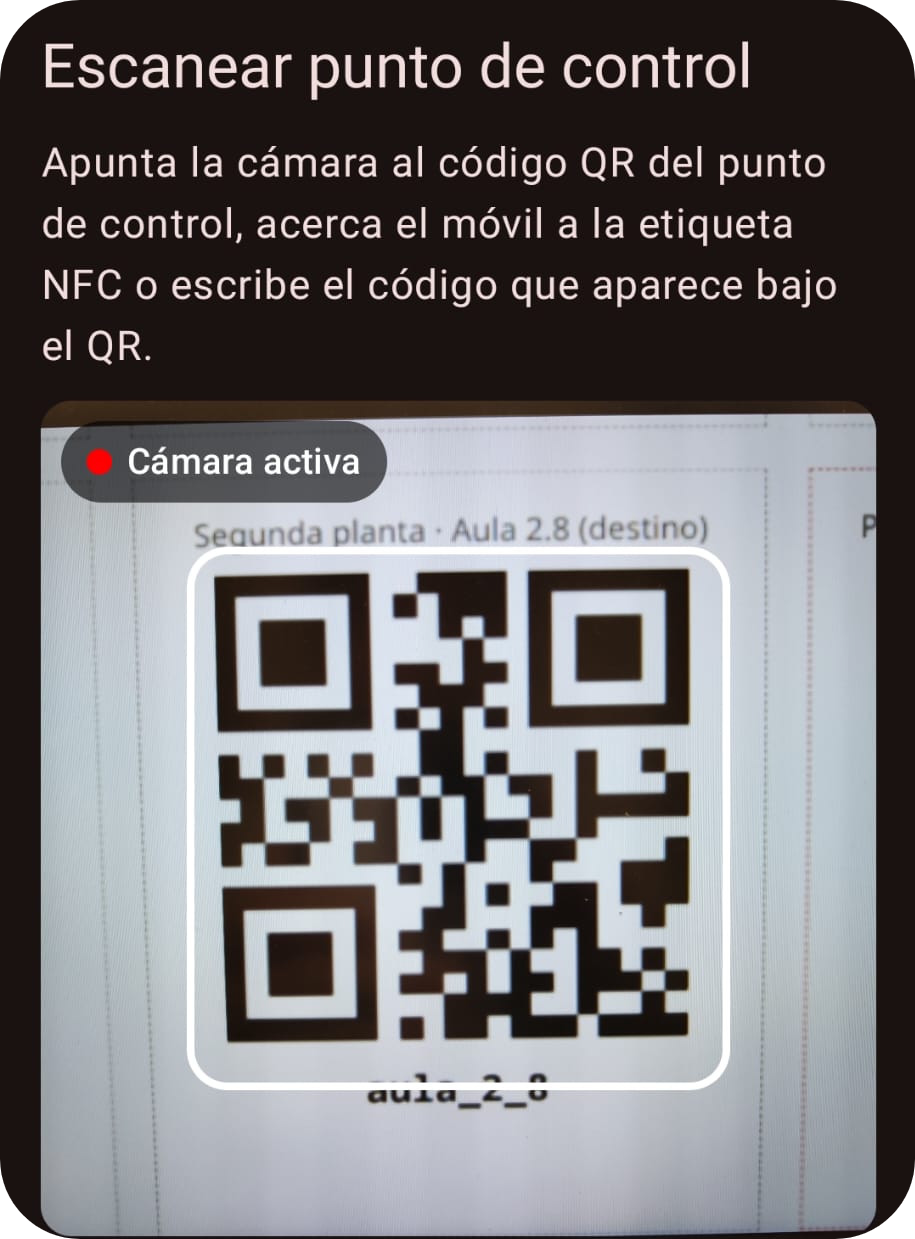
\includegraphics[width=3.5cm]{img/punto_control.png}
    %   \ph{4.6cm}{3.9cm}{pantalla del lector QR con el aviso «Cámara activa»}
  \end{columns}
  \vspace{2mm}
%   \begin{tikzpicture}
%     \node[fill=panel,rounded corners=5pt,inner sep=6pt,text width=13.1cm,font=\scriptsize]
%       {\textbf{Mismo texto en los tres:} el ID del nodo, p.\,ej. \code{escalera\_p0}.
%        Se trata como texto no confiable: solo \code{[A-Za-z0-9\_.-]}, de 1 a 64 caracteres y que exista en el catálogo.\\
%        \textbf{Punto equivocado $\rightarrow$ aviso y la ruta no avanza.}};
%   \end{tikzpicture}
  \presenta{Juan Antonio}
\end{frame}

% ============================================================
%  4. GESTO G1
% ============================================================
\begin{frame}{Gesto G1: asentir dos veces}
  \demo
  \centering
  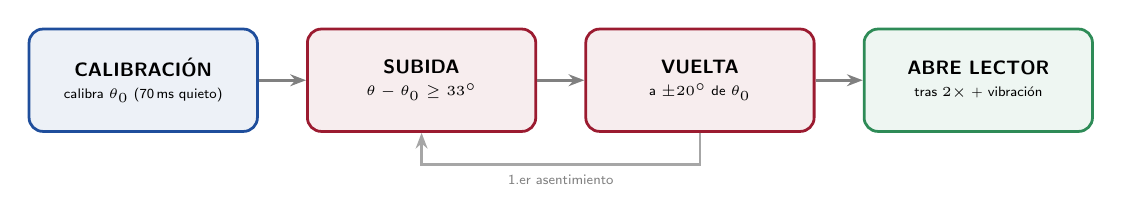
\begin{tikzpicture}[
      arr/.style={-{Stealth[length=2mm]},line width=1pt,gray}]
    \node[st=azul] (a) {\textbf{CALIBRACIÓN}\\\tiny calibra $\theta_0$ (70\,ms quieto)};
    \node[st=granate,right=6mm of a] (b) {\textbf{SUBIDA}\\\tiny $\theta-\theta_0\geq 33^\circ$};
    \node[st=granate,right=6mm of b] (c) {\textbf{VUELTA}\\\tiny a $\pm20^\circ$ de $\theta_0$};
    \node[st=verde,right=6mm of c] (d) {\textbf{ABRE LECTOR}\\\tiny tras $2\times$ + vibración};
    \draw[arr] (a)--(b); \draw[arr] (b)--(c); \draw[arr] (c)--(d);
    \draw[arr,gray!70] (c.south) -- ++(0,-4mm) -| node[pos=0.25,below,font=\tiny,text=gray]{1.er asentimiento} (b.south);
  \end{tikzpicture}
  \\[4mm]
  \begin{columns}[T]
    \column{0.37\textwidth}\raggedright
      \textbf{\color{granate}Cómo se detecta}\\[2pt]
      \footnotesize
      Sensor de gravedad (o acelerómetro filtrado) y ángulo de cabeceo
      $\theta=\operatorname{atan2}(g_y,g_z)\cdot\frac{180}{\pi}$.\\[2pt]
      Compara con la postura inicial, \textbf{sin giroscopio}: vale asentir rápido o despacio.
    \column{0.31\textwidth}\raggedright
      \textbf{\color{granate}No se reconoce}\\[2pt]
      \footnotesize
      \begin{itemize}\setlength\itemsep{1pt}
        \item Un solo asentimiento
        \item Subir menos de $33^\circ$
        \item Girar el móvil de lado
        \item Móvil vertical o boca abajo
      \end{itemize}
      Alternativa: botón «Escanear».
    \column{0.26\textwidth}
      \centering
    %   \ph{3.3cm}{3.2cm}{panel del gesto con el contador «1 de 2»}
      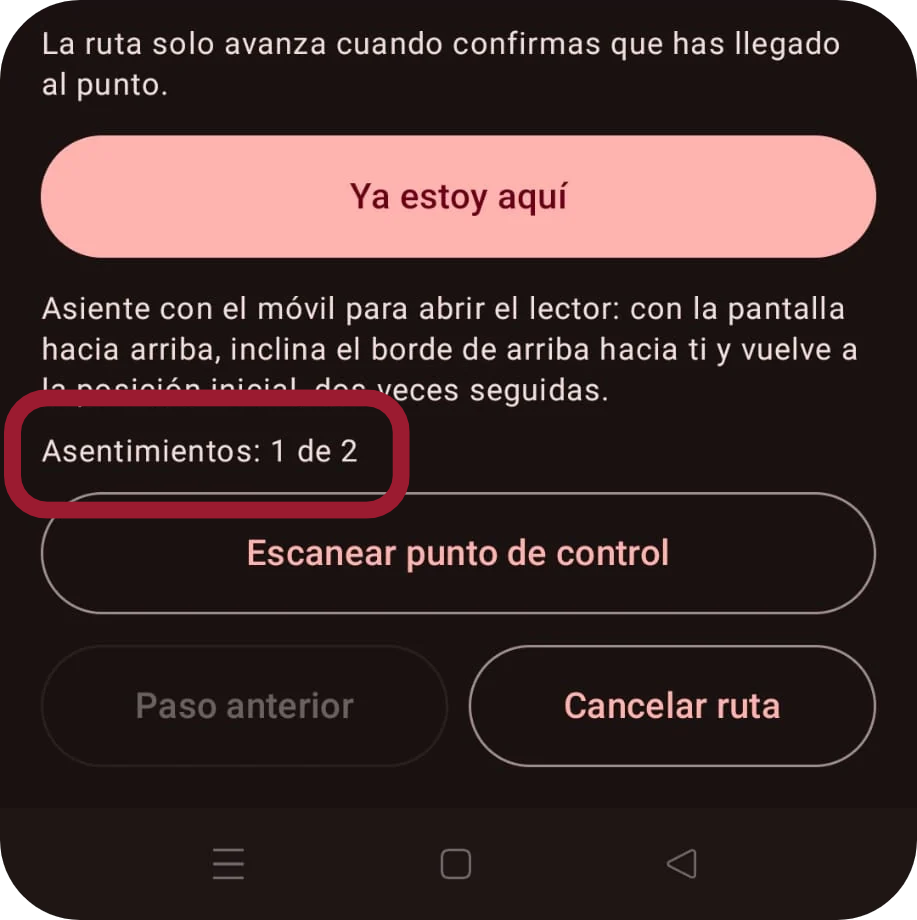
\includegraphics[width=3.5cm]{img/proceso_asentir.png}
  \end{columns}
  \presenta{José Manuel}
\end{frame}

% ============================================================
%  5. BRÚJULA, BARÓMETRO Y ESCUCHAR
% ============================================================
\begin{frame}{Brújula, barómetro y «Escuchar»}
  \demo
  \vspace{-1cm}
  \begin{columns}[T]
    \column{0.32\textwidth}\centering
    %   \ph{3.9cm}{1.9cm}{brújula «¿Voy bien?» con las dos flechas}\\[2mm]
        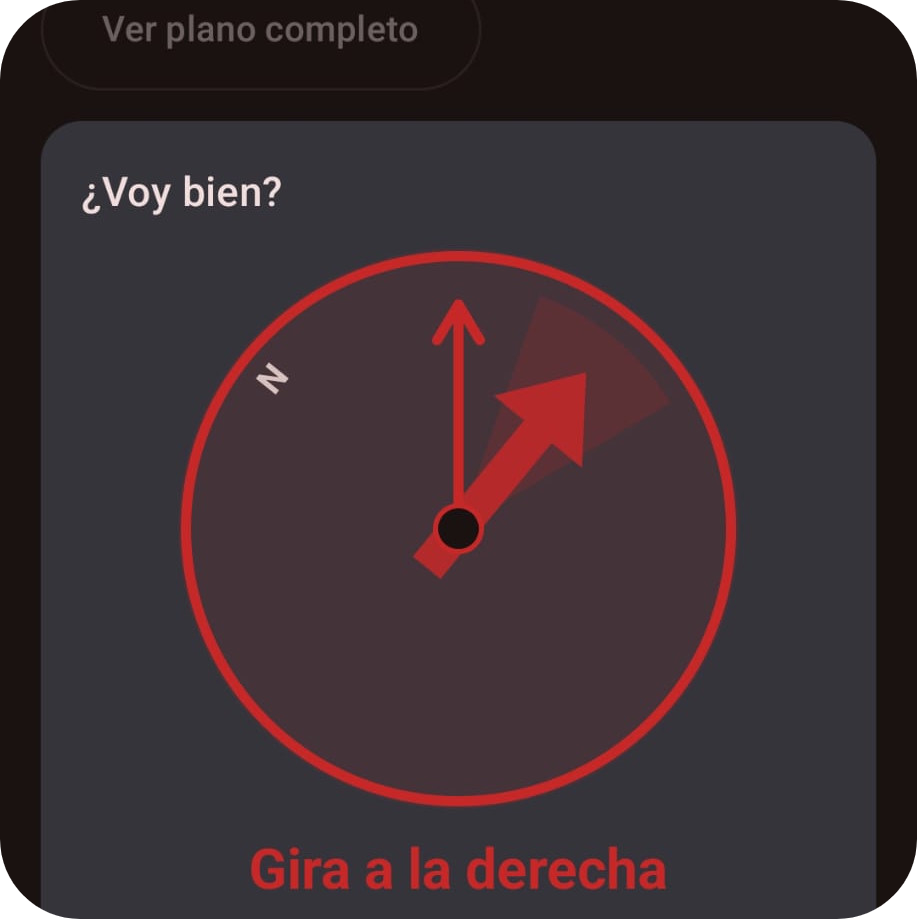
\includegraphics[width=3.5cm]{img/brujula.png}\\[2mm]
        \card{4.1cm}{2.2cm}{granate}{Vector de rotación}%
        {Compara hacia dónde apunta el móvil con el rumbo real del tramo.\\[1mm] ``Vas bien''/``Gira a la derecha''}
    \column{0.32\textwidth}\centering
      % \ph{3.9cm}{1.9cm}{aviso «Parece que ya estás en la segunda planta»}\\[2mm]
        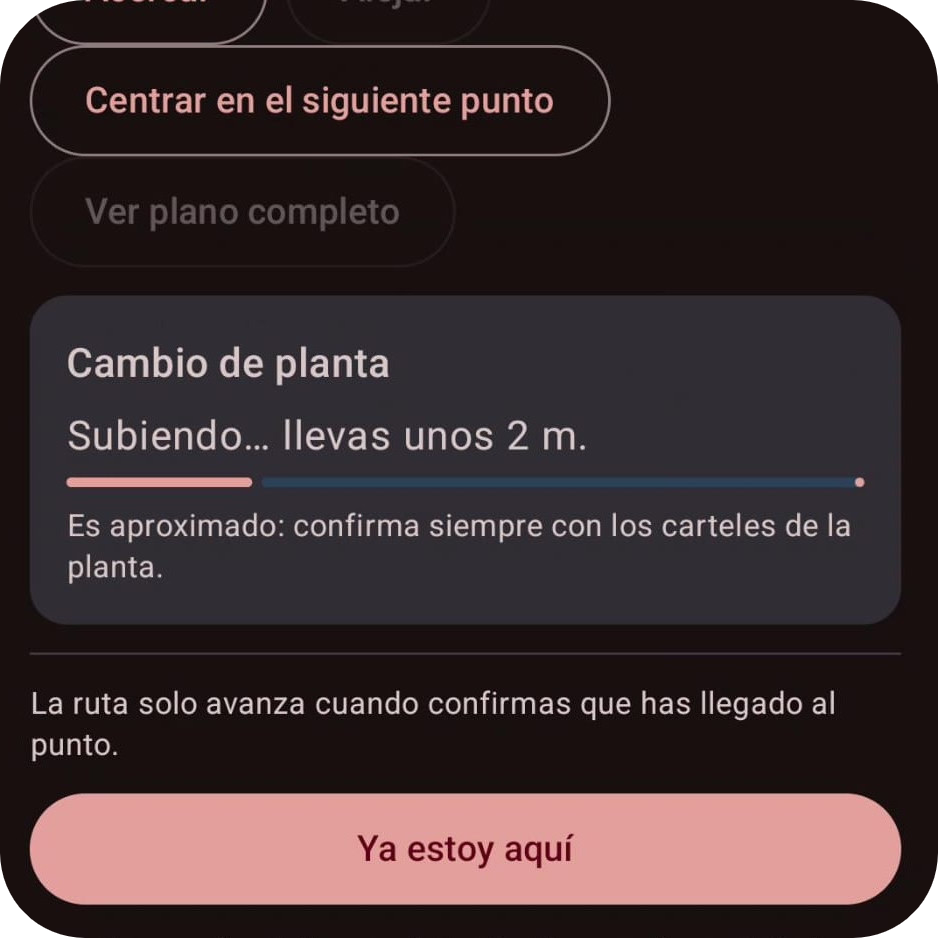
\includegraphics[width=3.5cm]{img/cambio_planta.png}\\[2mm]
        \card{4.1cm}{2.2cm}{azul}{Barómetro}%
        {En escalera y ascensor: la presión baja ${\approx}0{,}12$\,hPa por metro. Avisa del cambio de planta, pero \textbf{no avanza la ruta}.}
    \column{0.32\textwidth}\centering
    %   \ph{3.9cm}{1.9cm}{panel «Escuchar» con pausa / reanudar / parar}\\[2mm]
        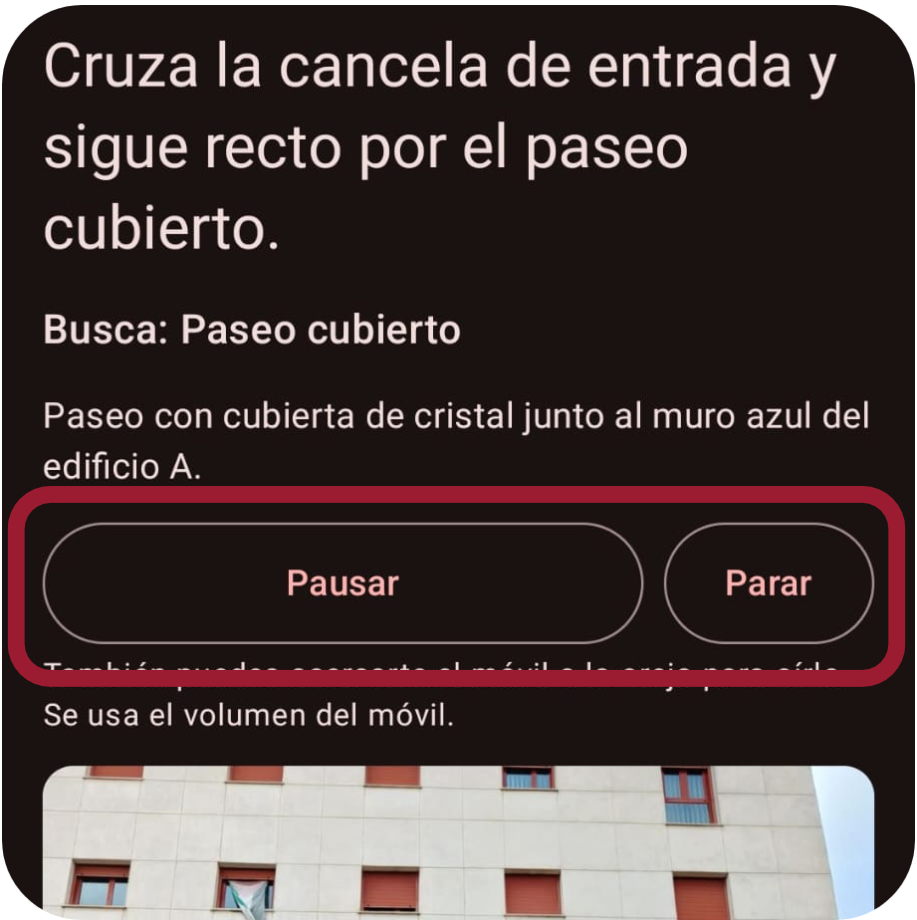
\includegraphics[width=3.5cm]{img/escuchar.png}\\[2mm]

        \card{4.1cm}{2.2cm}{verde}{Proximidad + voz}%
        {Acercar el móvil a la oreja lee el paso en voz alta (TextToSpeech). Pausa, reanudar y parar.}
  \end{columns}
  \vspace{0mm}
  \centering\scriptsize
%   \textbf{\color{granate}El color nunca va solo:} siempre hay texto, y todo es compatible con TalkBack.
  \presenta{Daniel \textperiodcentered{} Miguel (barómetro)}
\end{frame}

% ============================================================
%  6. ARQUITECTURA
% ============================================================
\begin{frame}{Arquitectura y decisiones de diseño}
  \begin{columns}[T]
    \column{0.57\textwidth}
      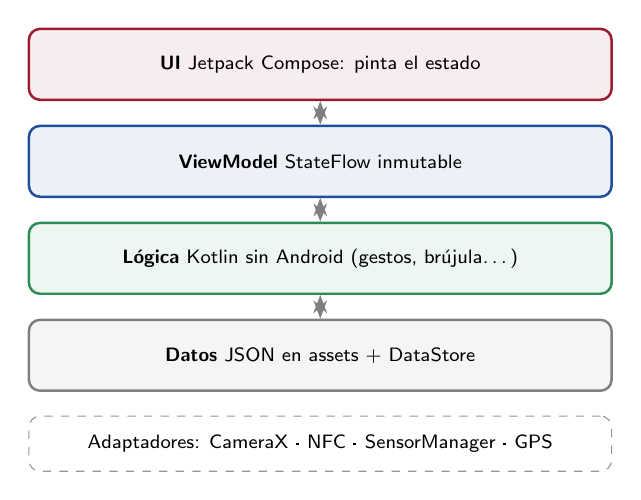
\begin{tikzpicture}[
          arr/.style={Stealth-Stealth,gray,line width=0.8pt}]
        \node[layer=granate] (ui) {\textbf{UI} \hfill Jetpack Compose: pinta el estado};
        \node[layer=azul,below=3mm of ui] (vm) {\textbf{ViewModel} \hfill StateFlow inmutable};
        \node[layer=verde,below=3mm of vm] (lg) {\textbf{Lógica} \hfill Kotlin sin Android (gestos, brújula\ldots)};
        \node[layer=gray,below=3mm of lg] (dt) {\textbf{Datos} \hfill JSON en assets + DataStore};
        \draw[arr] (ui)--(vm); \draw[arr] (vm)--(lg); \draw[arr] (lg)--(dt);
        \node[draw=ink!50,dashed,rounded corners=4pt,minimum width=7.4cm,minimum height=7mm,
              font=\scriptsize,below=3mm of dt] {Adaptadores: CameraX \textperiodcentered{} NFC \textperiodcentered{} SensorManager \textperiodcentered{} GPS};
      \end{tikzpicture}
    \column{0.40\textwidth}
      \footnotesize
      \textbf{\color{granate}Por qué así}
      \begin{itemize}\setlength\itemsep{3pt}
        \item \textbf{Sin servidor} ni permiso de Internet: todo funciona sin conexión.
        \item \textbf{JSON local}, no base de datos: los datos son fijos.
        \item \textbf{DI manual}, no Hilt: más simple para este tamaño.
        \item \textbf{Lógica sin Android}: se prueba sin móvil.
        \item Cada gesto tiene botón; interfaz ES/EN.
      \end{itemize}
  \end{columns}
  \presenta{Jesús}
\end{frame}

% ============================================================
%  7. RESULTADO, LIMITACIONES Y CONTINUACIÓN
% ============================================================
\begin{frame}{Resultado, limitaciones y continuación}
  \begin{columns}[T]
    \column{0.32\textwidth}
      \card{4.1cm}{3.5cm}{verde}{Resultado}%
        {8 sensores y modalidades de 5 categorías: visión, comunicación, táctil, movimiento, posición y entorno que trabajan en conjunto para orientar dentro y fuera de la escuela.\\[2pt]
         Probado en teléfonos reales.}
    \column{0.32\textwidth}
      \card{4.1cm}{3.5cm}{granate}{Limitaciones}%
        {%
            Solo hay una ruta de muestra (entrada $\leftrightarrow$ aula 2.2).\\[2pt]
            Cada móvil tiene sensores distintos y no son demasiado precisos.\\[2pt]
            La brújula solo es útil si sigues el tramo correcto.
        }
    \column{0.32\textwidth}
      \card{4.1cm}{3.5cm}{azul}{Cómo seguir}%
        {Más rutas: editar \code{graph.json} y añadir el QR del nodo.\\[2pt]
         Más espacios en \code{campus.json}; umbrales en \code{GestureConfig}.}
  \end{columns}
  \vspace{3mm}
 
  \presenta{José Manuel \textperiodcentered{} Jesús (cierre)}
\end{frame}

\end{document}